\section{Architecture and Proposed Approach}
\subsection{Three-tier architecture}
The system has device, edge, and cloud decision levels. A device executes
locally or sends a task to its fixed associated edge. The edge executes the
task or forwards it to a shared cloud scheduler. The cloud chooses a queue
discipline when a worker becomes available. The small simulator demonstration
uses three devices and two edges; the RL campaign instead uses 24 devices,
three edges, and one shared cloud. Device-to-edge associations are explicit,
not learned as arbitrary routing choices. The campaign association is
round-robin across the three edges, as shown in Fig.~\ref{fig:topology}.
The decision boundaries are shown in Fig.~\ref{fig:architecture}.

\begin{figure}[t]
\centering
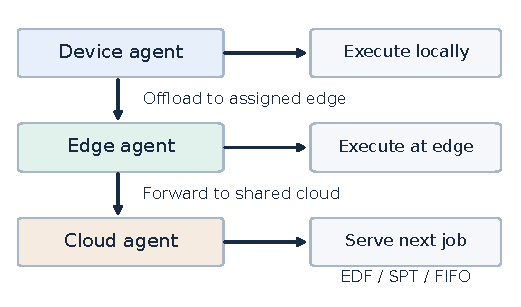
\includegraphics[width=\columnwidth]{figures/architecture.pdf}
\caption{Decision paths for the three agents. The device and edge can
execute at their own tier or escalate. The cloud chooses the service rule.}
\label{fig:architecture}
\end{figure}

\begin{figure}[t]
\centering
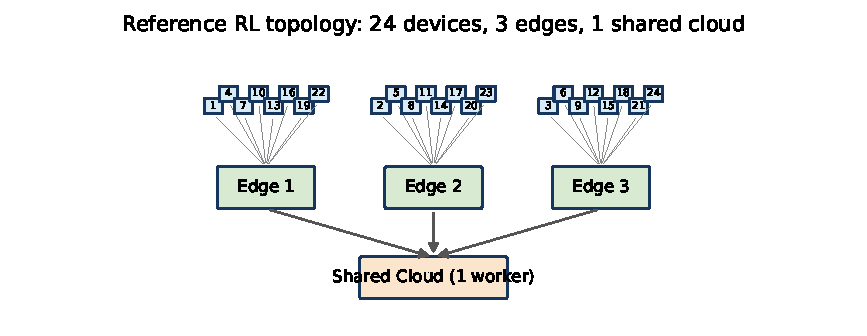
\includegraphics[width=\columnwidth]{figures/topology_24_devices.pdf}
\caption{Reference RL topology: 24 devices, three associated edges, and one
shared cloud worker.}
\label{fig:topology}
\end{figure}

\subsection{Task lifecycle and resource model}
The lifecycle is arrival, device decision, optional device--edge upload, edge
decision, optional edge--cloud upload, cloud dispatch, execution, and result
return. Queues contribute waiting time, and every modeled link contributes
serialization, propagation, and resource queue delay. Fig.~\ref{fig:lifecycle}
illustrates these paths.

\begin{figure}[t]
\centering
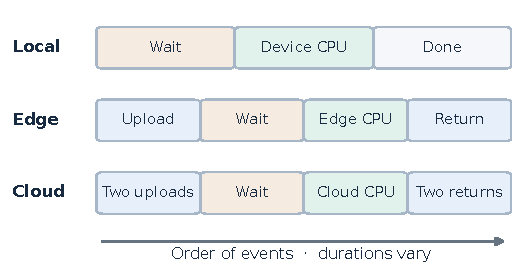
\includegraphics[width=\columnwidth]{figures/task_lifecycle.pdf}
\caption{Event order for the local, edge and cloud routes. Wait denotes
the compute queue. Transfers can also incur link queueing.}
\label{fig:lifecycle}
\end{figure}

Each task has arrival time, decimal-MB input and result sizes, required MI,
device identifier, relative deadline, and priority. For demand $w$ MI and
capacity $c$ MIPS,
\begin{equation}
t_{\mathrm{cpu}} = w/c.
\end{equation}
For payload $s$ decimal MB, bandwidth $B$ Mbps, propagation $p$, and queue
wait $q$,
\begin{equation}
t_{\mathrm{link}} = 8s/B+p+q.
\end{equation}
Latency is completion minus arrival, and a task meets its deadline when
$t_{\mathrm{completion}}\leq t_{\mathrm{arrival}}+D$. Devices and edges use
capacity-one SimPy resources. The current cloud has one worker and chooses
EDF, shortest processing time (SPT), or FIFO. Device energy includes CPU
energy per MI and transmit/receive power times radio duration; idle,
reception-infrastructure, retransmission, and cloud energy are not modeled.

\subsection{Observations and actions}
The device observation contains normalized work, input size, deadline slack,
battery fraction, device capacity, device--edge link state, and an optional
delayed edge-congestion signal. Its actions are local execution and edge
offloading. The edge observes task demand and deadline, edge queue/utilization,
edge capacity, edge--cloud link state, and an optional delayed cloud signal.
Its actions are edge execution and cloud forwarding. The cloud observes queue
length, deadline summaries, estimated service time, oldest wait, the count
of near-deadline jobs and workload imbalance. Device, edge and cloud use
11, 10 and 11 features. Work is log-scaled to compress its heavy tail.
The cloud chooses EDF (earliest absolute deadline), SPT (shortest
estimated service), or FIFO (first arrival to the cloud queue).
A centralized comparator uses a 16-feature
global observation and selects device, edge, or cloud, with fixed EDF cloud
dispatch. Lower-tier hierarchical agents do not receive raw global state.

\subsection{Learning and reward}
Q-learning estimates how much reward an agent can expect from an
action and the decisions that follow. For a policy $\pi$, the
action value is
\begin{equation}
Q^\pi(s,a)=
\mathbb E_\pi\!\left[\sum_{k=0}^{\infty}\gamma^k r_{t+k}
\mid s_t=s,\ a_t=a\right].
\end{equation}
Here $s$ is the observation used for control, $a$ is the action,
and $r_t$ is the reward assigned to the current decision. A
tabular Q-learning update adjusts the value of the observed pair
toward a target that combines the immediate reward and the best
estimated next action \cite{watkins1992}.
\begin{equation}
Q(s,a)\leftarrow Q(s,a)+
\alpha\left[r+\gamma\max_bQ(s',b)-Q(s,a)\right].
\end{equation}
The learning rate $\alpha$ controls the correction. At episode
termination the future term is zero.

Our observations include continuous quantities such as remaining
deadline, battery and queue wait. A table would require discretizing
their combinations. Deep Q-learning approximates $Q(s,a)$ with a
neural network. A Deep Q-Network (DQN) returns one score per
discrete action in a single pass. Fig.~\ref{fig:qnetwork} shows the
architecture used at each tier. The controller explores during
training and chooses the highest-scoring action during evaluation.

\begin{figure}[t]
\centering
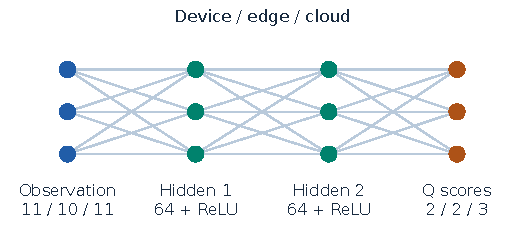
\includegraphics[width=\columnwidth]{figures/q_network.pdf}
\caption{DQN architecture shared by design across the three tiers.
Each controller has its own learned weights and input/output sizes.}
\label{fig:qnetwork}
\end{figure}

The DQN and Double DQN agents use two hidden layers of 64 units, replay
capacity 8,000, batch size 32, learning rate $3\mathord{\times}10^{-4}$,
target updates every 500 optimization steps, and Smooth L1 loss. Double DQN
selects the next action with the online network and evaluates it with the
target network. DQN takes the target-network maximum. Splitting selection
and evaluation addresses the upward bias that can arise when choosing
the largest of several noisy estimates \cite{hasselt2016double}.

For non-cloud decisions, the shared task reward is
\begin{equation}
\begin{aligned}
R=-\bigg(&w_l\min\left(1,\frac{\log(1+L/D)}{\log(10001)}\right)
+w_e\min\{3,E/E_0\}\\
&+w_d\mathbb{1}[\mathrm{miss}]
+w_c\min\{3,F/F_0\}\bigg),
\end{aligned}
\end{equation}
with $(w_l,w_e,w_d,w_c)=(0.35,0.25,0.35,0.05)$. Here $L$, $D$, $E$, and
$F$ denote end-to-end latency in seconds, deadline in seconds, device energy
in joules, and feedback bytes. The implementation uses $E_0=0.3$ J and
$F_0=64$ bytes from the default \texttt{RewardWeights} configuration; these
are normalization references, not measured campaign means. The miss indicator
is one when a deadline-feasible task misses its deadline. These weights
are design choices that trade off latency, device energy, feasible
deadline misses and feedback cost in a common scalar. The logarithm
compresses large latency ratios. In $\log(10001)$, the number 10,001
is $1+10{,}000$. At $L/D=10{,}000$, the normalized latency penalty
reaches one, and clipping caps it there. For example, with $L=2$ s,
$D=1$ s, $E=0.15$ J, $F=32$ B and a nominally feasible deadline, the
four weighted penalties are about 0.042, 0.125, 0.350 and 0.025.
The reward is their negative sum, approximately $-0.542$.
The cloud uses a
queue-waiting-cost reward for contested dispatches, so its objective is not
identical to the shared task reward.

The task reward is computed after completion and assigned to the decisions
on its route. The evaluated protocol links consecutive observations in each
controller's decision log, with $\gamma=0.9$ and a terminal transition
at the end of the log. Consecutive decisions can concern different tasks.
For reward $r$ and next observation $s'$, DQN uses
$y=r+\gamma\max_a Q_{\mathrm{target}}(s',a)$.
Double DQN selects $a^*=\arg\max_a Q_{\mathrm{online}}(s',a)$ and uses
$y=r+\gamma Q_{\mathrm{target}}(s',a^*)$. Both use $y=r$ at the final
transition.

The cloud reward is $-\min\{1,\log(1+n\hat t)/\log(10001)\}$,
where $n$ is the queue size at dispatch and $\hat t$ is the estimated
service duration in seconds. This proxy for queue occupancy during
service favors shorter jobs at a given queue size. Singleton queues are
omitted from cloud replay because the three rules select the same job.
\subsection{Feedback}
Feedback is adjacent-tier and causal. A snapshot sampled at time $t$ is
available only after modeled propagation and serialization, at a later
decision. Conditions are none, periodic, frequent, and event-triggered. The
event trigger sends an initial snapshot, sends when the signal change reaches a
threshold, and refreshes after five observations. Feedback bytes, modeled
delay, and information age are recorded. At a decision, information age is
the elapsed time since the consumed snapshot was sampled \cite{yatesAoI}.
The modeled control path operates independently of data-plane queues. Fig.~\ref{fig:coordination} shows this control path.

\begin{figure}[t]
\centering
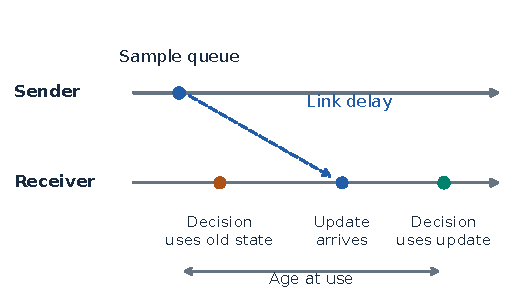
\includegraphics[width=\columnwidth]{figures/coordination.pdf}
\caption{Timing of a queue snapshot sent to the neighboring tier.
Information age is measured from sampling to the decision that uses it.}
\label{fig:coordination}
\end{figure}
